\chapter{System Identification}
\label{ch:ch2}

In the preceding chapter, a model-dependent, differentially flat controller was introduced for the control of an eVTOL aircraft. In order for that controller to work outside of simulation in hardware, the aerodynamic model of the aircraft needs to be very accurate. That is, the mathematical aircraft model must closely approximate the physical aircraft. If this is not the case, the autopilot will internally calculate forces and moments which do not accurately correspond to the actual forces and moments on the aircraft. 

Recall from chapter \ref{ch:VTOL} in Equations \ref{eq:totalAerodynamicForcesMoments} for aerodynamic Forces and Moments. These equations are an approximation of the true forces and moments experienced by this aircraft. These equations are utilized by the controller to produce certain desired forces and moments on the aircraft. For example, recall section \ref{sec:momentControl} in chapter \ref{ch:VTOL}, where elevator moment control was discussed. For a given $M_{des}$ input, this section found the best possible $\delta_e$ in an attempt to match that desired moment to reality. 

If the aerodynamic coefficients for pitch moment ($C_{M_0},C_{M_\alpha},C_{M_q},C_{M_{\delta_e}}$) are not accurate, an incorrect $\delta_e$ may be calculated. 
If this control input has an error that is too large, then the aircraft may become unstable, which is especially true during the transition phase.

One may ask how these aerodynamic coefficients are to be calculated to begin with. 
One method would be to use aerodynamic modelling using CAD modelling and aerodynamic software. 
As our lab continues development of 3D printed aircraft, this solution is probably the best way forward as the 3D CAD model is readily available.
Another would be wind tunnel experimentation and data collection. This is only feasible for relatively small airframes that can fit inside of the available wind tunnels.
Finally, flight data can be processed and analyzed to create an estimate for the aerodynamic coefficients.
This final option is possible if a general aerodynamic model of the aircraft exists and is accurate, and only the specific numbers for aerodynamic coefficients must be estimated.

In this section, we develop a method of estimating coefficients of aerodynamics gathered from flight data using a recursive least squares (RLS) algorithm.

\section{Aerodynamic Coefficients}

While the VTOL model in chapter \ref{ch:VTOL} only included longitudinal, or vertical, coefficients of aerodynamics in table \ref{tb:longitudinalCoefficients}, all autopilots will be benefited by a better model of the aircraft, including standard airplane models. For this reason, we also estimate the lateral coefficients of aerodynamics, shown in table \ref{tb:lateralCoefficients}.


\begin{table}
\label{tb:longitudinalCoefficients}
\centering
\caption{Longitudinal Aerodynamic Coefficients for Airplane}
\begin{tabular}{|c !{\vrule width 1.2pt} c !{\vrule width 1.2pt} c|}
    \hline
    $C_{L_0}$ & $C_{D_0}$ & $C_{m_0}$\\
    \hline
    $C_{L_\alpha}$ & $C_{D_\alpha}$ & $C_{m_\alpha}$\\
    \hline
    $C_{L_q}$ & $C_{D_q}$ & $C_{m_q}$\\
    \hline
    $C_{L_{\delta_e}}$ & $C_{D_{\delta_e}}$ & $C_{m_{\delta_e}}$\\
    \hline
\end{tabular}
\end{table}

\begin{table}
\label{tb:lateralCoefficients}
\centering
\caption{Lateral Aerodynamic Coefficients for Airplane}
\begin{tabular}{|c !{\vrule width 1.2pt} c !{\vrule width 1.2pt} c|}
    \hline
    $C_{Y_0}$ & $C_{l_0}$ & $C_{n_0}$\\
    \hline
    $C_{Y_\beta}$ & $C_{l_\beta}$ & $C_{n_\beta}$\\
    \hline
    $C_{Y_p}$ & $C_{l_p}$ & $C_{n_p}$\\
    \hline
    $C_{Y_r}$ & $C_{l_r}$ & $C_{n_r}$\\
    \hline
    $C_{L_{\delta_a}}$ & $C_{l_{\delta_a}}$ & $C_{n_{\delta_a}}$\\
    \hline
    $C_{L_{\delta_r}}$ & $C_{l_{\delta_r}}$ & $C_{n_{\delta_r}}$\\
    \hline
\end{tabular}
\end{table}




\section{Aerodynamic Modes}

\subsection{Phughoid Mode}

One common aerodynamic mode is called the phughoid mode. This effect is a vertical oscillation of the aircraft, as depicted in Fig. \ref{fig:phughoid_diagram}. When the aircraft's phughoid mode has been excited, the aircraft will pitch up, ascend slightly, lose airspeed, and then pitch down, gain airspeed, and descend slightly before repeating the process. In other words, the phughoid mode couples north velocity $\dot{n}$ with pitch $\theta$, and down position $d$. According to chapter 6 in \cite{flightDynamicsPrinciples}, this mode is relatively slow, and lightly damped, so it takes some time return to normal. When the aircraft goes through this, it will experience large signal changes in angle of attack $\alpha$, pitch angular rate $q$, pitch angular acceleration $\dot{q}$, north acceleration $\ddot{n}$, and down acceleration $\ddot{d}$. This mode is typically induced by quick impulses on the elevator. Excitation of this mode is useful as it may produce large signals from internal sensors for estimate of coefficients of aerodynamics. 


\begin{figure}
    \centering
    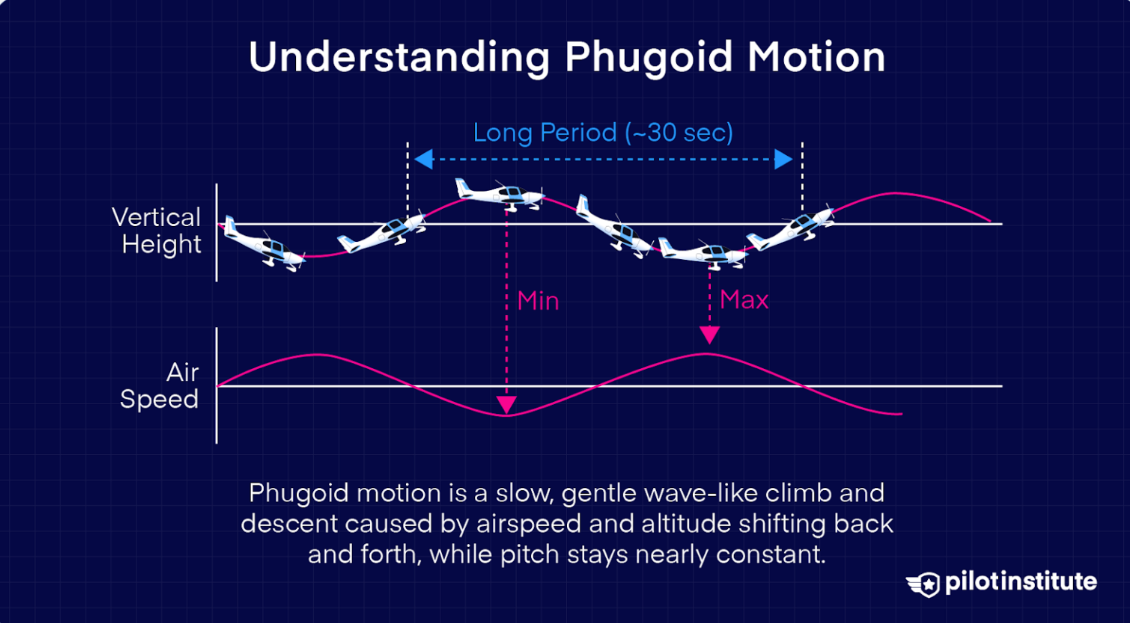
\includegraphics[width=0.5\linewidth]{figs/chap2/phughoid_mode_diagram.png}
    \caption{Illustration of phugoid motion showing oscillations in altitude and airspeed over time. Image by Pilot Institute, from ``Phugoid Motion in Aviation: What It Is and Why It Matters'' (2025). \cite{pilotinstitute_phugoid}}
    \label{fig:phughoid_diagram}
\end{figure}


\subsection{Dutch Roll Mode}

Another common aerodynamic mode is called dutch roll, which is a coupling of both yaw and pitching moments, as described in \cite{cookLateralDirectionalDynamics}. 
That is, the aircraft oscillates between yawing sharply, rolling sharply as yaw returns to zero, and then repeating in the other directions, according to chapter 7 of \cite{flightDynamicsPrinciples}. This means that after an aircraft has rolled to the left and it returns upright, the aircraft will yaw to the right, which will cause the aircraft to roll to the right, which will repeat the process. Just as excitation of the phughoid mode created large longitudinal signals, dutch roll creates large lateral signals. For example, the the two roll moments $l$ and $n$ cause large signals for $p$, $r$, $\dot{p}$, and $\dot{r}$. Large yaw $\psi$ maneuvers will also create large signals for east acceleration $\ddot{e}$ and sideslip angle $\beta$. Intentional excitation of this mode is generally accomplished by rudder impulses, though this may also be enhanced with delayed aileron impulses.

\begin{figure}
    \centering
    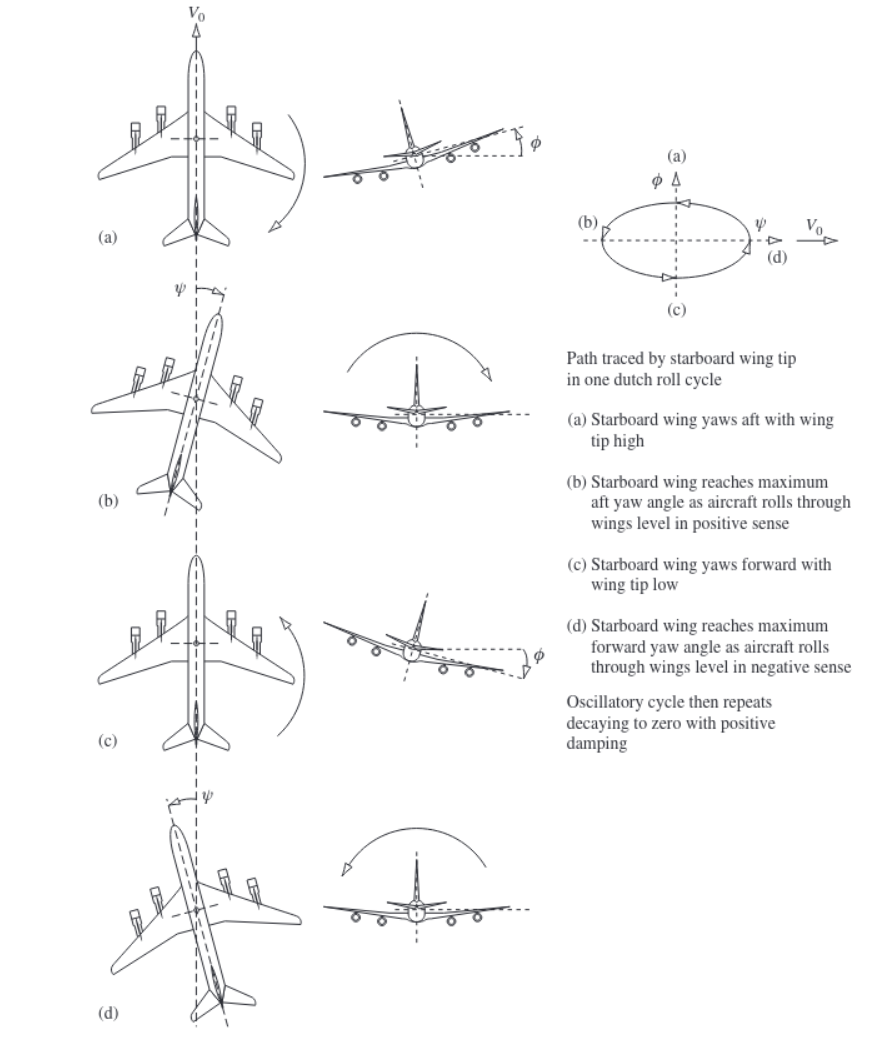
\includegraphics[width=0.7\linewidth]{figs/chap2/Dutch Roll Diagram.png}
    \caption{Dutch roll oscillation of an aircraft. Reproduced from Fig. 7.5 in Flight Dynamics \cite{flightDynamicsPrinciples}}
    \label{fig:dutchRollDiagram}
\end{figure}

These modes are generally undesirable for aircraft to experience during normal flight. For aircraft with less stable airframes, inducing such modes pushes the aircraft closer to instability. Such large oscillations may also cause motion sickness for passengers and crew. However, such maneuvers tend to excite the  aerodynamic characteristics, which means that the signal associated with each aerodynamic coefficient can become large enough to distinguish it from the other generated signals.

\section{Recursive Least Squares}

While sensor data is being collected from the aircraft, an algorithm  must run to calculate the coefficients of aerodynamics. Such an algorithm would make the best estimate of the coefficients of aerodynamics, based on the acquired data. For this reason, the recursive least squares (RLS) filter was selected. The following explanation or derivation of an RLS filter is an adaptation of lecture slides created by \citeauthor{beardRLS} in \cite{beardRLS}.

\subsection{RLS Derivation}

The equation for an Infinite Impulse response (IIR) system, with $n$ poles and $m+1$ zeroes is shown in \ref{eq:Difference} and is shown graphically in Fig. \ref{fig:IIR}. In a standard IIR filter setup, a signal $x_n$ is the time series input to the system and $y_n$ is the time series output of the system. The coefficients $a_i$ scale time delayed outputs $y_n$ of the system, and the coefficients $b_i$ scale time delayed inputs $x_n$ of the system. The input signal $x_n$, $b_i$ coefficients, and $a_i$ coefficients are known quantities. The IIR filter then generates the output signal $y_n$ using these known values for each timestep.

\begin{align}
    y[k] = a_1 y[k-1] + \hdots + a_n y[k-n] + b_0 u[k] + \hdots + b_m u[k-m] + \eta_k
    \label{eq:Difference}
\end{align}

\begin{figure}
    \centering
    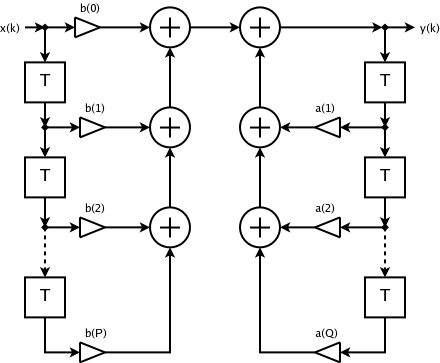
\includegraphics[width=0.5\linewidth]{figs/chap2/IIR-filter.png}
    \caption{IIR Filter Diagram. Image by Mwilde, licensed under CC BY-SA 3.0 \cite{IIRfilterImage}}
    \label{fig:IIR}
\end{figure}

In the case of an LMS filter, the $a_i$ and $b_i$ coefficients are unknown, while the input $x_n$ and output $y_n$ signals are known. The goal is to estimate these scaling coefficients $a_i$ and $b_i$ using data from input and output. In other words, the LMS filter estimates the coefficients of an IIR filter, or a system that is approximated as an IIR filter, as shown in Fig. \ref{fig:LMSEstimatingIIR}.

\begin{figure}
    \centering
    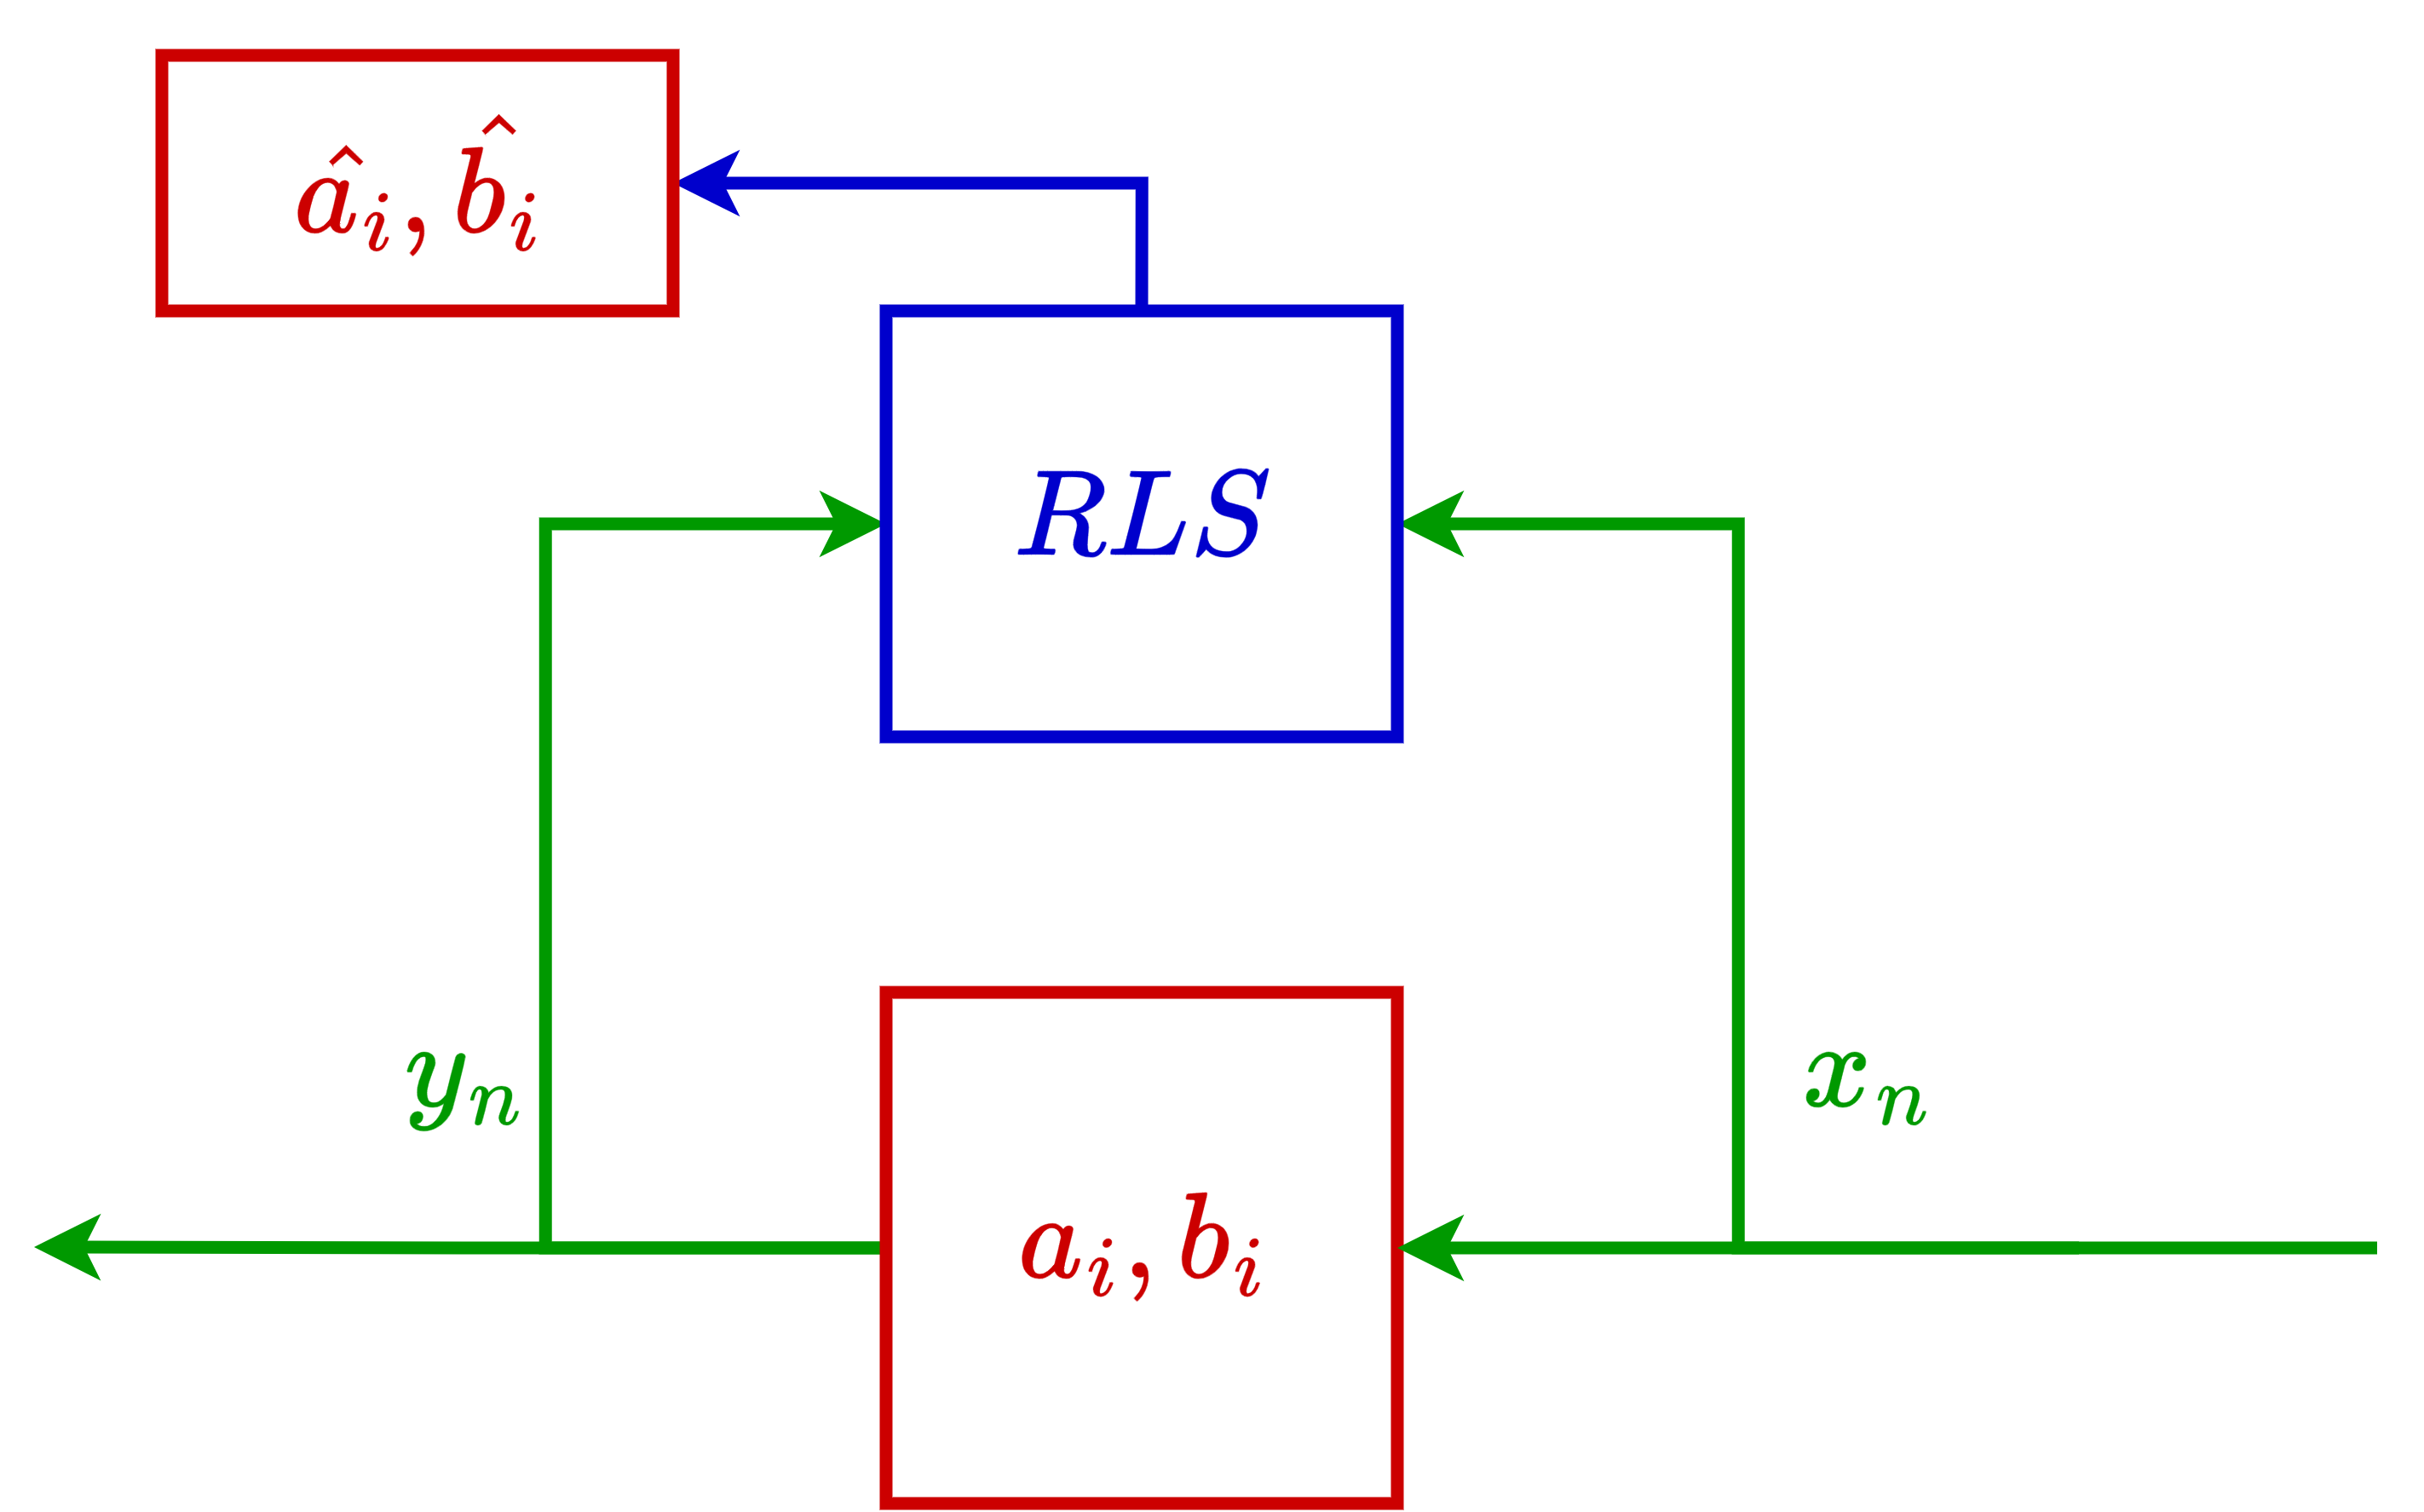
\includegraphics[width=0.5\linewidth]{figs/chap2/Input Output Black Box.drawio.png}
    \caption{An LMS filter estimating the coefficients of aerodynamics output from a system approximated by an IIR filter.}
    \label{fig:LMSEstimatingIIR}
\end{figure}

Equation \ref{eq:Difference} is represented in matrix form in Eq. 

\begin{align}
    y[k] = \bs{a}_k^\top \bs{x} + \eta_k \\
\end{align}
Where:
\begin{align}
    \bs{a}_k^\top =
    \begin{bmatrix}
        y[k-1] & \hdots & y[k-n] & u[k] & \hdots & u[k-m]
    \end{bmatrix}\\
    \bs{x}^\top =
    \begin{bmatrix}
        a_1 & \hdots & a_n & b_0 & \vdots & b_m
    \end{bmatrix}^\top
\end{align}

Where $\eta$ represents a random variable as noise added to the system. The vector $\bs{a}_k^\top$ represents a window of $n$ samples of $y[k]$ and $m+1$ samples of input $u[k]$. Each new sample $k$ is a new shifted $\bs{a}_k^\top$ vector with a corresponding output $y[k]$. These shifted $y[k]$, $a_k$, and $\eta_k$ vectors can be stacked into the following matrix form.

\begin{align}
    \begin{bmatrix}
        y[1]\\
        \vdots\\
        y[N]\\
    \end{bmatrix}
    =
    \begin{bmatrix}
        \bs{a}_1^\top\\
        \vdots\\
        \bs{a}_N^\top\\
    \end{bmatrix}
    \bs{x}_N
    +
    \begin{bmatrix}
        \eta_1\\
        \vdots\\
        \eta_N\\
    \end{bmatrix}
\end{align}

And can be represented as:

\begin{align*}
    \bs{y}_N = A_N \bs{x}_N + \bs{\eta}_N\\
    \bs{y}_N =
    \begin{bmatrix}
        y[1]\\
        \vdots\\
        y[N]\\
    \end{bmatrix}
    \text{,}
    \quad
    A_N =
    \begin{bmatrix}
        \bs{a}_1^\top\\
        \vdots\\
        \bs{a}_N^\top\\
    \end{bmatrix}
    \text{,}
    \quad
    \bs{\eta}_N =
    \begin{bmatrix}
        \eta_1\\
        \vdots\\
        \eta_N\\
    \end{bmatrix}
\end{align*}

\subsection{Batch Least Squares}

For a complete set of matrices, the least squares solution is found using the left pseudoinverse of the form:

\begin{align*}
    \bs{x}^*_N = \left(A_N^\top A_N\right)^{-1} A_N^\top \bs{y}_N\\
\end{align*}

This is the mathematical solution for this problem. However, a large matrix inverse like this would be prohibitively expensive to recalculate. This equation would have to be recalculated at each time step, which would be a prohibitively large $\mathcal{O}(n^3)$ operation. We need an algorithm that only performs a pseudoinverse once, and uses a recursive formula to perform a much smaller computation at each time step afterwards.

\subsection{Recursive Algorithm}

Given: 
\begin{align*}
    \bs{x}^*_N = \left(A_N^\top A_N\right)^{-1} A_N^\top \bs{y}_N\\
\end{align*}

Define:
\begin{align*}
    P_N = \left(A_N^\top A_N\right)^{-1}\\
    \bs{z}_N = A_N^\top \bs{y}_N\\
\end{align*}

For the previous sample of $N-1$, where $A_n$ is one row shorter:

\begin{align}
    A_{N-1} = 
    \begin{bmatrix}
        \bs{a}_0^\top\\
        \vdots\\
        \bs{a}_{N-1}^\top
    \end{bmatrix}\\
    P_{N-1}^{-1} = A_{N-1}^\top A_{N-1} =
    \begin{bmatrix}
        \bs{a}_1 \hdots \bs{a}_{N-1}
    \end{bmatrix}
    \begin{bmatrix}
        \bs{a}_1^\top\\
        \vdots\\
        \bs{a}_{N-1}^\top
    \end{bmatrix}
    =\sum_{i=1}^{N-1} \bs{a}_i \bs{a}_i^\top
\end{align}

So then for the current sample
\begin{align}
    P_N^{-1} = \sum_{i=1}^{N} \bs{a}_i \bs{a}_i^\top = 
    \bs{a}_N \bs{a}_N^\top +\sum_{i=1}^{N-1} \bs{a}_i \bs{a}_i^\top
    = P_{N-1}^{-1} + \bs{a}_N \bs{a}_N^\top
\end{align}

So, $P_N^{-1}$ is just the previous matrix $P_{N-1}^{-1}$ plus the update $\bs{a}_N \bs{a}_N^\top$. We want to find the inverse of this matrix: $P_N$, which is:

\begin{align*}
    P_N = \left( P_{N-1}^{-1} + \bs{a}_N \bs{a}_N^\top\right)^{-1}
\end{align*}

Now, the matrix inversion Lemma provides a shortcut as:

\begin{align}
    P_N = P_{N-1} - P_{N-1} \bs{a}_N \bs{a}_N^\top P_{N-1} \left(I + \bs{a}_N^\top P_{N-1} \bs{a}_N\right)^{-1}
\end{align}

Which simplifies the inverse to the inverse of a 1x1 matrix, which is significantly more computationally efficient and stable than an (n+m)x(n+m) matrix inverse.


Similarly,

\begin{align}
  \bs{z}_N = A_N^{\top} \bs{y}_N\\
  =\Sigma_{i=1}^N \bs{a}_i y[i]\\
  =\left(\Sigma_{i=1}^{N-1} \bs{a}_i y[i] + \bs{a}_N y[N] \right)\\
= \bs{z}_{N-1} + \bs{a}_N y[N]\\
\end{align}

With these tools, we can rewrite the least squares solution as

\begin{align}
    \bs{x}_N = (A_N^\top A_N) A_N^{\top} \bs{y}_N\\
    = P_N \bs{z}_N\\
    = \left(P_{N-1} - \frac{P_{N-1}\bs{a}_N \bs{a}_N^\top P_{N-1}}{1 + \bs{a}^{\top}P_{N-1} \bs{a}_N} \right) \left(\bs{z}_{N-1} \bs{a}_N y[N]\right)
\end{align}

Define that Kalman gain as:

\begin{align}
  \bs{k}_N = \frac{P_{N-1} \bs{a}_N}{1 + \bs{a}_N^\top P_{N-1} \bs{a}_N}
\end{align}


\section{Coefficient Equations for Fixed Wing Aircraft}

\label{sec:equationsOfMotion}

The equations for each set of coefficients are given in the following sections. All of the original equations are found in Small Unmanned Aircraft: Theory and Practice \cite{uav_book}. The equations for Lift, Drag and y forces are given in 4.3, 4.4, and 4.14 in \cite{uav_book} respectively. The equations for moments about the x, y, and z axes are given in 4.15, 4.5, and 4.16 respectively. For example, the equation for forces in the y direction is given as:

\begin{align}
    f_y = \frac{1}{2} \rho V_a^2 S \left[ C_{Y_0} + C_{Y_\beta} \beta + C_{Y_p} \frac{b}{2 V_a} p + C_{Y_r} \frac{b}{2 V_a} r + C_{Y_{\delta_a}} \delta_a + C_{Y_{\delta_r}} \delta_r\right]
\end{align}

Similar equations exist for the two other forces and three other moments. These equations are for a standard Fixed-Wing aircraft, as found in the Mavsim simulation environment.

\subsection{Y Coefficients}

\begin{align}
    a_n = \frac{1}{2m} \rho V_a^2 S
    \begin{bmatrix}
        1 & \beta & \frac{b}{2V_a}p & \frac{b}{2V_a}r & \delta_a & \delta_r
    \end{bmatrix}\\
    y_n =
    \begin{bmatrix}
        \ddot{y}
    \end{bmatrix}
\end{align}

\subsection{Lift and Drag Coefficients}

\begin{align}
    a_n = \frac{1}{2m} \rho V_a^2 S
    \begin{bmatrix}
        s_{\alpha} & -c_{\alpha}\\
        -c_{\alpha} & -s_{\alpha}\\
    \end{bmatrix}
    \begin{bmatrix}
        1 & \alpha & \frac{c}{2 V_a} q & \delta_e & 0 & 0 & 0 & 0\\
        0 & 0 & 0 & 0 & 1 & \alpha & \frac{c}{2 V_a} q & \delta_e\\
    \end{bmatrix}\\
    y_n =
    \begin{bmatrix}
        \ddot{x}\\
        \ddot{z}\\
    \end{bmatrix}
    -
    \begin{bmatrix}
        \frac{T(\delta_t, V_a)}{m}\\
        0\\
    \end{bmatrix}
\end{align}

Note that the signal $y_n$ for lift and drag must subtract thrust generated by the forward rotor.

\subsection{l Estimator}

\begin{align}
    a_n = \frac{1}{2} \rho V_a^2 S b
    \begin{bmatrix}
        1 & \beta & \frac{b}{2V_a} p & \frac{b}{2V_a}r & \delta_a & \delta_r
    \end{bmatrix}\\
    y_n = 
    \begin{bmatrix}
        J_x \dot{p} - J_y q r + J_z q r - J_{xz} \dot{r} - J_{xz} p q
    \end{bmatrix}
\end{align}

\subsection{m Estimator}

\begin{align}
    a_n = \frac{1}{2} \rho V_a^2 S c
    \begin{bmatrix}
        1 & \alpha & \frac{c}{2 V_a} q & \delta_e
    \end{bmatrix}\\
    y_n = 
    \begin{bmatrix}
        J_y \dot{q} + J_x p r + J_{xz} p^2 - J_z p r - J_{xz} r^2
    \end{bmatrix}
\end{align}

\subsection{n Estimator}

\begin{align}
    a_n = \frac{1}{2} \rho V_a S b
    \begin{bmatrix}
        1 & \beta & \frac{b}{2V_a} p & \frac{b}{2V_a} r & \delta_a & \delta_r
    \end{bmatrix}\\
    y_n = 
    \begin{bmatrix}
        -J_x p q + J_y p q + J_z \dot{r} - J_{xz} \dot{p} + J_{xz} q r
    \end{bmatrix}
\end{align}

\subsection{A Note on Gravity}

A confusing part of this problem is gravity. We naturally assume in the paper that acceleration due to gravity is given as:

\begin{align}
    a_{g_{3D}} =
    \begin{bmatrix}
        0\\
        0\\
        9.81
    \end{bmatrix}
    \quad
    a_{g_{2D}} =
    \begin{bmatrix}
        0\\
        9.81\\
    \end{bmatrix}
\end{align}

However, because all components of the accelerometer are equally influenced by gravitational acceleration, it is impossible to discriminate a gravitational field. If an accelerometer is placed on a table, it will sense the normal force of $9.81 \frac{m}{s^2}$ in the upwards direction. In the same manner, if the aircraft is flying in trim, level flight with no acceleration, the accelerometer will sense the Lift force as $9.81 \frac{m}{s^2}$ in the up direction. Gravity is then entirely removed from all aerodynamic sensing equations.

\section{2D VTOL Equations}

The equations for a 2D VTOL are somewhat modified from a standard aircraft; they do not include y forces, nor l and n moments. There is also the addition of two vertical rotors. This modifies the equations of motion to be the following. It is easiest to group the x and z forces into the same category, because they are linked to Lift and Drag forces, which are functions of angle of attack.

\subsection{Lift And Drag}

\begin{align}
    x =
    \begin{bmatrix}
        C_{L_0} & C_{L_\alpha} & C_{L_q} & C_{L_{\delta_e}} & C_{D_0} & C_{D_\alpha} & C_{D_q} & C_{D_{\delta_e}}
    \end{bmatrix}^\top\\
    a_n = \frac{1}{2m} \rho V_a^2 S
    \begin{bmatrix}
        s_\alpha & -c_{\alpha}\\
        -c_{\alpha} & -s_{\alpha}\\
    \end{bmatrix}
    \begin{bmatrix}
        1 & \alpha & \frac{c}{2 V_a} q & \delta_e & 0 & 0 & 0 & 0\\
        0 & 0 & 0 & 0 & 1 & \alpha & \frac{c}{2 V_a} q & \delta_e\\
    \end{bmatrix}\\
    y_n =
    \begin{bmatrix}
        \ddot{z_x}\\
        \ddot{z_z}\\
    \end{bmatrix}
    - \frac{1}{m}
    \begin{bmatrix}
        T(\delta_{t,forward})\\
        -T(\delta_{t,front}) - T(\delta_{t,rear})\\
    \end{bmatrix}
\end{align}

\subsection{m moment}

\begin{align}
    x =
    \begin{bmatrix}
        C_{m_0} & C_{m_\alpha} & C_{m_q} & C_{m_{\delta_e}}
    \end{bmatrix}^\top\\
    a_n = \frac{1}{2} \rho V_a^2 S c
    \begin{bmatrix}
        1 & \alpha & \frac{c}{2V_a} q & \delta_e
    \end{bmatrix}\\
    y_n = 
    \begin{bmatrix}
        J_y \dot{q}
    \end{bmatrix}
    =
    \begin{bmatrix}
        J_y \ddot{\theta} - (T(\delta_{t_{front}}) - T(\delta_{t_{rear}}))
    \end{bmatrix}
\end{align}

Note that $y_n$ simplifies significantly in this equation because all rotational inertia values besides $J_y$ are all zero. Also please note the subtraction of all forces and moments caused by the three rotors.


\section{Input Signals}

There must be sufficient excitation of the aircraft for the LMS filter to converge on stable values. The values of $y_n$ and the components in $a_n$ for each of the 5 estimators have sufficiently large magnitudes to overcome noise and other internal parasitic signals. If the aircraft flies solely in trimmed level flight, the LMS filter will not converge on stable or accurate values. There must also be a significant variation in the corresponding values to set the columns of $A$ as linearly independent. Sufficiently large control surface inputs are required for this. This usually means creating a series of square wave impulses for each of the control surfaces: aileron $\delta_a$, elevator $\delta_e$, and rudder $\delta_r$. 

Phughoid mode is induced by impulses of elevator control input, which excites the vertical dynamics of the aircraft. Similarly, Dutch roll mode is induced by the impulses of the aileron and rudder, though the best results happen when there is a separation between the aileron control input and the rudder control input.

\section{MAVSIM Results}

Mavsim is a Python flight simulator package that was developed for testing flight dynamics and control. The main simulation in Mavsim is an airplane with the same aerodynamic equations of motion as described in section \ref{sec:equationsOfMotion}. That is, it is a standard airplane with 30 coefficients of aerodynamics, with 12 longitudinal coefficients and 18 lateral coefficients.

An LMS filter specific to this aircraft model was written. When the aircraft is flying during a simulation, the applicable flight data, as specified in the above sections, is passed into the LMS filter and run recursively.

The control input signal for elevator $\delta_e$ control is shown in Fig. \ref{fig:phughoidControlInput} and the control input signals for aileron $\delta_a$ and rudder $\delta_r$ are shown in Fig. \ref{fig:dutchRollControlInput}. It turns out that the best control input for the elevator we could find was a chirp signal, which is a sine wave of steadily increasing frequency. This corresponded well to the aircraft's phughoid mode oscillation. 

When the elevator maneuver is completed, the dutch roll is performed, For the dutch roll mode, both rudder and aileron control input were used. Each impulse lasts $0.2$ seconds total, where the control $\delta_a$ or $\delta_r$ is $0.3$ for $0.1$ seconds and $-0.3$ for $0.1$ seconds. That is, each impulse has an equal positive and then negative component. The signals are two-sided because a one-sided control in the aileron signal causes the aircraft to roll around, which is unstable for flight. Each maneuver is repeated six times for each control surface, with a delay of $2.0$ seconds between impulses. The entire maneuver lasts approximately $25.0$ seconds.

It is worth noting that dutch roll can be induced with rudder alone. However, the aerodynamic coefficients corresponding to $\delta_a$ ($C_{Y_{\delta_a}}$, $C_{l_{\delta_a}}$, $C_{n_{\delta_a}}$) would not be excited with $\delta_a = 0$. Therefore, both control surfaces are utilized. 

\begin{figure}
    \centering
    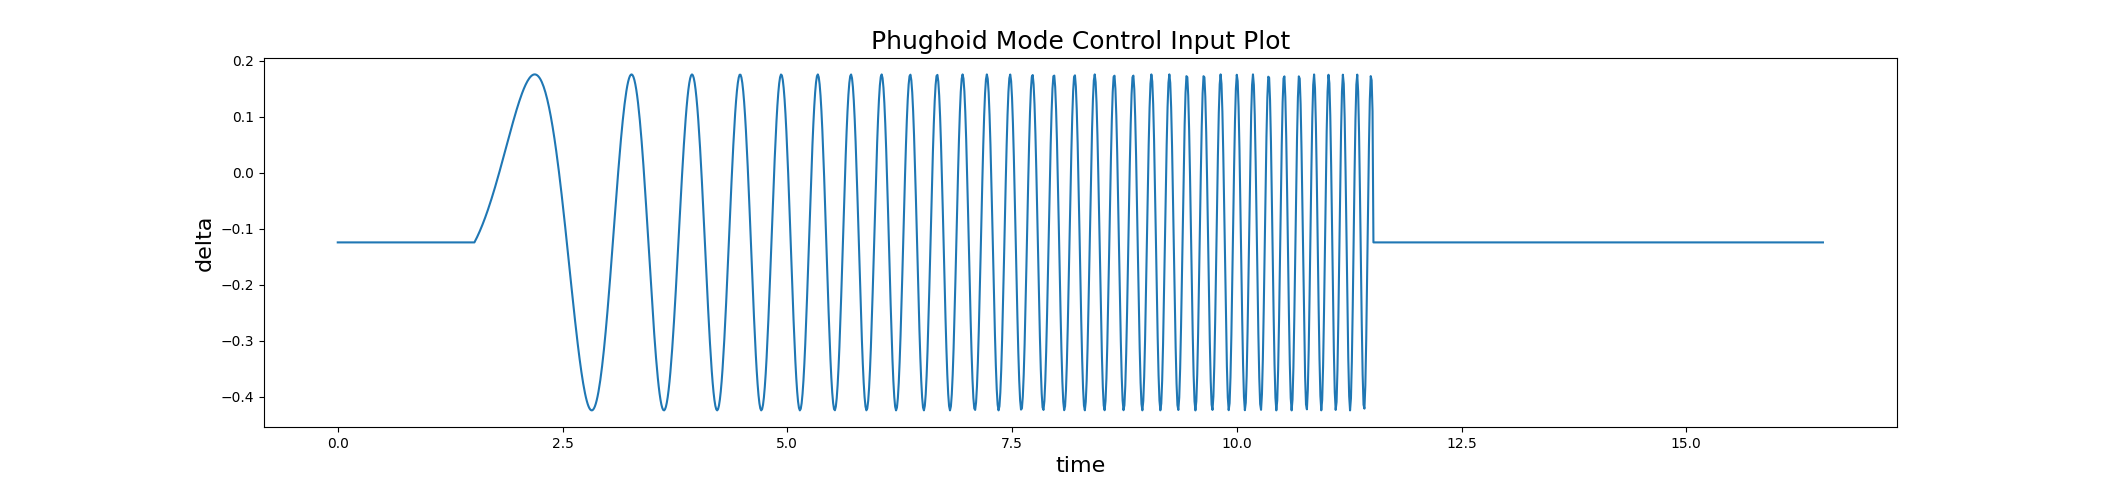
\includegraphics[width=1.0\linewidth]{figs/chap2/Phughoid Mode Control Input Plot 2.png}
    \caption{Elevator Control Input for excitation of Phughoid Mode in MAVSIM Aerodynamic Coefficient Estimation}
    \label{fig:phughoidControlInput}
\end{figure}

\begin{figure}
    \centering
    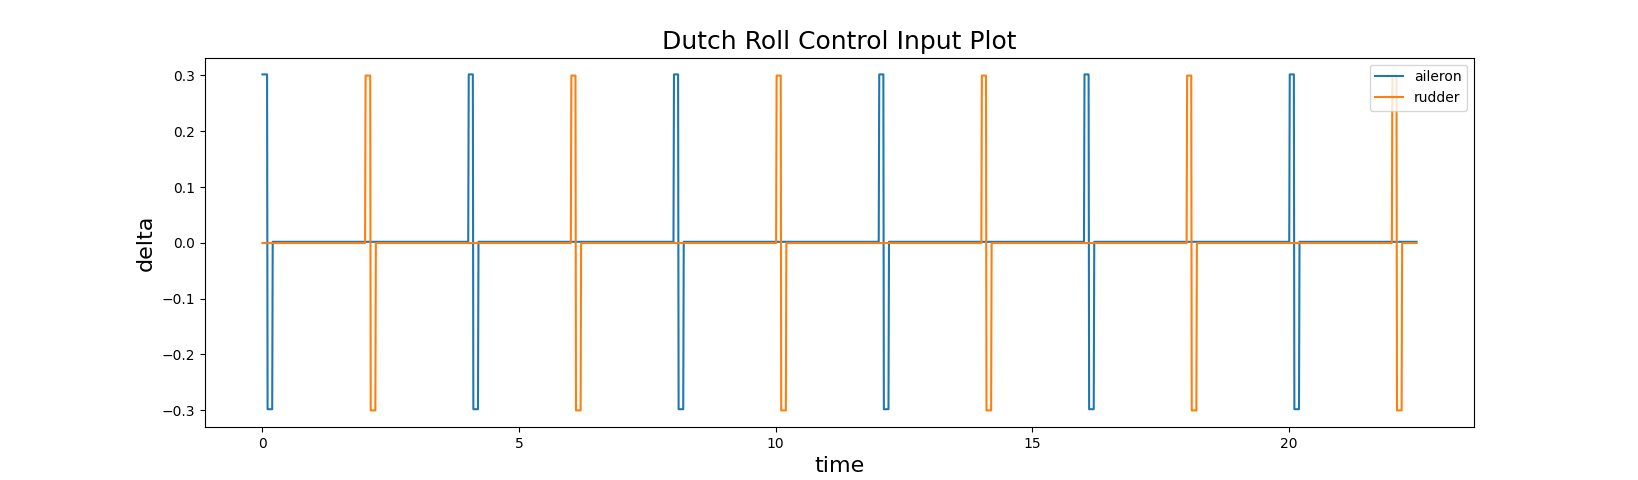
\includegraphics[width=1.0\linewidth]{figs/chap2/Dutch roll control Inputs Plot 2.png}
    \caption{Aileron and Rudder Control Input for excitation of Dutch Roll Mode in Mavsim Aerodynamic Coefficient Estimation}
    \label{fig:dutchRollControlInput}
\end{figure}

These open loop control signals cause the aircraft to deviate from the original direction. After each maneuver is completed, the autopilot engages and the aircraft returns to its original stable trajectory. Videos of the Mavsim flight simulation for coefficient estimation are found at: \href{https://youtube.com/shorts/tUv_ZsYx78U?feature=share}{Simulation Video} and \href{https://youtu.be/tRkiyvk2C58}{Signals Video}.

\subsection{Coefficient Comparison Table}

The following table contains all of the actual coefficients of aerodynamics compared to the coefficients calculated using the LMS filter, from the previous section. The error and error percentage are also given for each aerodynamic coefficient. 

\begin{table}[ht]
\centering
\caption{Mavsim Coefficients} % <-- caption first
\label{tb:Mavsim_Coefficients} % <-- label after caption
\begin{tabular}{|c|c|c|c|c|c|}
    \hline
    \csvreader[
        no head,
        table head=\hline,
        late after line=\\\hline
    ]{csvFiles/coefficients.csv}{1=\one,2=\two,3=\three,4=\four,5=\five,6=\six}
    {\two & \three & \four & \five & \six}
\end{tabular}
\end{table}

%The table with all of this information can be found at: https://docs.google.com/spreadsheets/d/1DW3H2LaMANrdXDkPXQFCwfoodEIRIJS1OVjl9R6R920/edit?usp=sharing


\section{ROSFlight Flight Data Results}

In August of 2025, we worked with the Rosflight team to obtain actual flight data from one of their flights. This was performed on an Anaconda Airframe as shown in Fig. \ref{fig:anaconda}. 




\section{Limitations}

This work is only a crude beginning. There are several important limitations for the implementation. 

\subsection{Noise}
The most obvious limitation for this sort of signal processing endeavor, as with all signal processing endeavors, is always noise. Noise is a pervasive parasite which was not assumed in these simulations.

\subsection{Nonlinear Modelling}

One of the challenges with a simplified model of the flight controller is that while the aircraft's coefficients of aerodynamics stay approximately constant within a small angle of attack, they are actually functions of the state, and are not entirely linear. 

Perhaps the most important coefficients for the VTOL project are those associated with pitch, such as $C_{L \alpha}$ and $C_{D \alpha}$. They are really functions of $\alpha$ as $C_L(\alpha)$ and $C_D(\alpha)$. The amount of lift depends on the localized angle of attack. 

\subsection{Design}

Another problem is the design of the eVTOL itself. With the addition of the booms for the vertical rotor, and the rotors themselves, this can significantly affect the aerodynamic model of the aircraft. This discrepancy will become more poignant in the future with future hardware implementation of the VTOL. The drag caused by the rotors during forward flight is of particular concern, an the drag model may need to be updated with extra coefficients to take this into account 

\subsection{Safety}

For hardware implementation, safety mechanisms in code will also need to be implemented. Boundaries will need to be drawn, and if the controller exceeds those boundaries, the safest fail safe will probably be to enter quadrotor mode again, and thereby remain in a safe flight regime.

\subsection{Calibration}

It may also be necessary for a differentially flat autopilot to work for the aircraft to fly some initial flights in standard fixed-wing flight and perform the maneuvers discussed above, in order to have a good estimation of the coefficients of aerodynamics beforehand. Without this calibration step, the differentially flat controller may make grave errors with calculations, and thereby increase the chance of failure dramatically.

\subsection{Hardware Implementation}


\begin{figure}
    \centering
    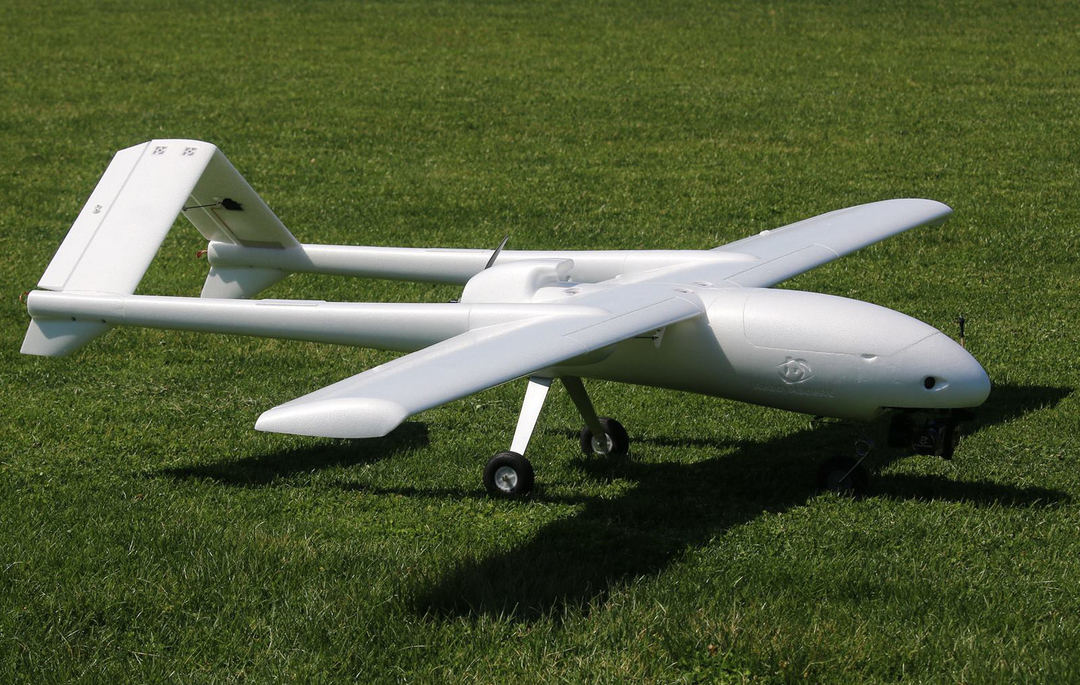
\includegraphics[width=0.5\linewidth]{figs/chap2/anaconda111.jpg}
    \caption{Ready Made RC - Anaconda Airframe}
    \label{fig:anaconda}
\end{figure}

Another airframe we want to develop a better model for is called the anaconda airframe, as shown in Fig. \ref{fig:anaconda}. 
This airframe is the primary platform for the development of Rosplane for the Rosflight autopilot stack. 
There is no current model of this airframe and it is desirable for the development of this autopilot to know those coefficients. 
Having this information will help with development and better tuning the autopilots.

Plenty of flight data has been gathered from autopilot test flights for Rosflight.
This flight data includes airspeed, accelerometer, gyroscope, and other related sensor and estimate data.
Originally, we had intended to use this flight data and implement it in the algorithm described previously.
However, it quickly became apparent that the estimates for angle of attack $\alpha$, and sideslip angle $\beta$ are inaccurate.
Accurate estimates of 

\section{Conclusion}

During an aircraft's flight, it is subject to 

While this preliminary work demonstrates the potential of an RLS algorithm for calculating coefficients of aerodynamics, there are actually many other implementations that already exist.
That is to say, there already exist several other open source code repositories that perform system identification on aircraft. 
While this implementation focuses solely on coefficients these other tools contain additional tools, including transfer function estimation, full state space modelling, and frequency response estimation.
One such tool was developed at ETH Zurich, and is available at \href{https://github.com/ethz-asl/data-driven-dynamics}{ETH Zurich Repo}.

In the future, this 
